% -------------------------------------------------------------------------------- %

\begin{exercise}[Autonomous Orchard]

\phantom{}

An AI controlled orchard needs to decide when to harvest its trees. To do this it measures the concentration
of three chemicals in the air. Each day the orchard can choose to wait or harvest. Waiting costs one credit in
operating costs while a harvest ends the process. Once a crop is harvested, packaged and sold, the orchard is
told the profit or loss of that harvest. Most experts agree that the function mapping the chemical concentrations
to the profit is linear with some error. The orchard has several samples of the profits from other harvests:

\begin{figure}[H]
    \centering
    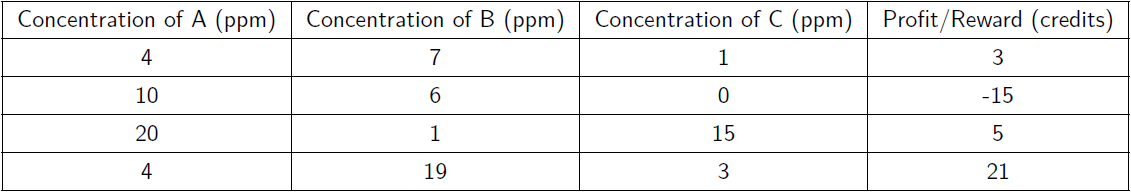
\includegraphics[width = 0.8 \textwidth]{9.1.png}
\end{figure}

Begin to approximate (by hand) the function that maps the state feature vector to Q(state, harvest) using an
MC goal. Do a gradient decent step on each sample. A sensible learning rate would be around 0.01, but feel
free to try any value.
\end{exercise}

% -------------------------------------------------------------------------------- %

\begin{solution}

We assume a linear value function with three-dimensional weight vector $\textbf{w} = (w_1,w_2,w_3)$
and feature vectors $\textbf{x}(s) = (x_1(s), x_2(s), x_3(s))$.

\begin{align*}
    \hat{v}(\textbf{s}, \textbf{w}) = x_1(s)w_1 + x_2(s)w_2 + x_3(s)w_3.
\end{align*}

We initialize the weight vector $\textbf{w}_0 = (0,0,0)$.

Applying the first gradient decent step with the given MC goal and $\alpha = 1/100$ yields

\begin{align*}
    \textbf{w}_1 &= \textbf{w}_0 + \alpha 
    \left[G_t - \hat{v}(S_1, \textbf{w}_0)\right]\nabla_{\textbf{w}}\hat{v}(S_1, \textbf{w}_0) \\
    &= (0,0,0) + \frac{1}{100}[3 - 0] \cdot (4,7,1) \\
    &= \frac{1}{100}(12,21,3).
\end{align*}

In the second step we obtain

\begin{align*}
    \textbf{w}_2 &= \frac{1}{100}(12,21,3) + \frac{1}{100}
    \left[-15 - \frac{1}{100}(12 \cdot 10 + 6 \cdot 21 + 0 \cdot 3)\right]
    \cdot (10, 6, 0) \\
    &= \frac{1}{100}(12,21,3) - \frac{1746}{10000}(10, 6, 0) \\
    &= \frac{1}{10000}(-16260,-8376,300) \\
    &\approx (-1.6, -0.8, 0)
\end{align*}

Finally after the third and fourth MC-update we end up with approximately

\begin{align*}
    \textbf{w}_3 &= (-1.6, -0.8, 0) + 
    \frac{1}{100}\left[5 + 1.6\cdot 20 + 0.8 \cdot 1 - 0 \cdot 15\right]
    \cdot (20, 1, 15) \\
    &= (-1.6, -0.8, 0) + \frac{37.8}{100}\cdot (20, 1, 15) \\
    &= \frac{1}{100}(596, -42.2, 567) \\
    &\approx (6.0, -0.4, 5.7) \\
    \textbf{w}_4 &= (6.0, -0.4, 5.7) +
    \frac{1}{100}\left[21 - 6.0 \cdot 4 + 0.4 \cdot 19 - 5.7 \cdot 3\right]
    \cdot (4, 19, 3) \\
    &= (6.0, -0.4, 5.7) - \frac{12.5}{100}\cdot (4, 19, 3) \\
    &= \frac{1}{100}(550, -277.5, 532.5) \\
    &\approx (5.5, -2.8, 5,3).
\end{align*}

\end{solution}

% -------------------------------------------------------------------------------- %
